%
%==> Section: Plotting functions
%
\section{
  Plotting functions
}
%
%==> Plotting user-defined functions
%
\begin{frame}[fragile]
  \frametitle{
    Plotting user-defined functions
  }

  Ti$k$Z also has a math engine which enables you to plot functions:

  \lstinputlisting{./tex/src/plot_function.tex}

  gives you

  \begin{center}
    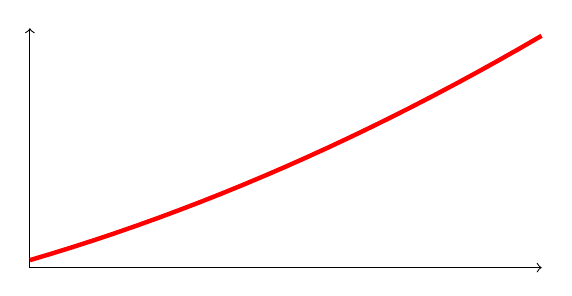
\begin{tikzpicture}[xscale=13,yscale=3.8]
  \draw [<->] (0,0.8) -- (0,0) -- (0.5,0);
  \draw[red, ultra thick, domain=0:0.5]
  plot (\x, {0.025+\x+\x*\x});
\end{tikzpicture}

  \end{center}

  The domain instruction shows the range of $x$ which is plotted. In this case we are plotting the function $0.025+x+x^2.$ Note the braces around the function that we plot in

  \begin{lstlisting}
    plot (\x, {function});
  \end{lstlisting}
  
\end{frame}

%
%==> Built-in math functions
%
\begin{frame}[fragile]
  \frametitle{
    Built-in math functions
}

  \begin{itemize}
  \item
    Many mathematical functions are possible; you will probably have enough with

    \begin{lstlisting}
      factorial(\x), sqrt(\x), exp(\x), ln(\x)
      log2(\x), log10(\x), abs(\x)
    \end{lstlisting}

  \item
    
    \begin{lstlisting}
      pow(\x,y), mod(\x, y)
    \end{lstlisting}

    which gives $x^y$ and $x$ modulo $y.$

  \item
    
    \begin{lstlisting}
      round(\x), floor(\x), ceil(\x)
    \end{lstlisting}
       
    rounds $x$ to the nearest integer, the largest integer smaller than $x$, the smallest integer larger than $x$.
  \end{itemize}
\end{frame}


%
%==> Built-in math functions (continued)
%
\begin{frame}[fragile]
  \frametitle{
    Built-in math functions (continued)
}

  \begin{itemize}
  \item
    \begin{lstlisting}
      sin(\x)
    \end{lstlisting}

    it assumes that $x$ is in degrees; if $x$ is expressed in radians use

    \begin{lstlisting}
      sin(\x r)
    \end{lstlisting}

    In a similar fashion,
    
    \begin{lstlisting}
      cos(\x), cos(\x r), tan(\x), tan(\x r)
    \end{lstlisting}

    We also have

    \begin{lstlisting}
      min(\x,y), max(\x,y).
    \end{lstlisting}
    
  \item 
    In mathematical expressions the two following \textcolor{violet}{\bf rational} variables can be useful:

    \begin{lstlisting}
      e
    \end{lstlisting}
    
    which is equal to \textcolor{violet}{2.718281828}, and

    \begin{lstlisting}
      pi
    \end{lstlisting}

    which is equal to \textcolor{violet}{3.141592654}.

  \end{itemize}
\end{frame}

%
%==> Plot trig functions
%
\begin{frame}[fragile]
  
  You can mix functions to compute more complicated expressions (see above for the reason for the {\tt r} parameter in the argument of $\sin$ and $\cos$ and note the use of \textcolor{violet}{\tt pi} to define the domains):
  \lstinputlisting{./tex/src/plot_trig_functions.tex}

  which gives you

  \begin{center}
    \input{./tex/src/plot_trig_functions.tex}
  \end{center}

\end{frame}
